\documentclass[a4paper]{article}
\usepackage{graphicx}
\usepackage{multirow}
\usepackage[table,xcdraw]{xcolor}
\usepackage{float}
\usepackage{amsmath}
\usepackage{bm}
\graphicspath{{diagrams/}}

\title{\textsc{CS760: Machine Learning Exam Review}} % Title
\author{
$$Jack Truskowski$$ \\
} 

\date{3/31/2018}

\begin{document}
\maketitle

\section{Topics}

\begin{enumerate}
\item Decision Tree Learning
\item Instance-based Learning, K-Nearest Neighbor
\item ML Methodology
\item Linear and Logistic Regression
\item Bayesian Network Learning
\item Neural Networks
\item Deep Neural Networks
\item Learning Theory
\item Support Vector Machines
\end{enumerate}

\section{Decision Tree Learning}
\subsection{Goals}
\begin{itemize}
\item DT representation
\item Standard approach
\item Occam's razor
\item Entropy / IG
\item Types of DT Splits
\item Test sets / unbiases accuracy estimates
\item Overfitting
\item Pruning
\item Tuning (validation) sets
\item Regression trees
\item m-of-splits
\item Lookahead
\end{itemize}

\subsection{Notes}
\begin{itemize}
\item Splits on nominal features have one branch per value
\item Splits on continuous features use a threshold
\item Candidate Splits on continuous features
  \begin{itemize}
  \item sorts the values
  \item split thresholds in intervals between different classes
  \end{itemize}
  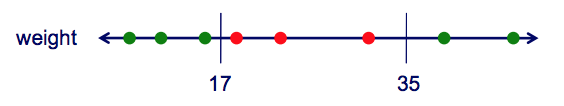
\includegraphics{contsplit}
\item The simplest tree with accurate classification will be the best
  on unseen data
\item \textbf{Occams razor}: Simpler models are better
\item IG Limitation: biased towards tests with many outcomes
\item Avoiding overfitting:
  \begin{enumerate}
  \item Early stopping: stop if further splitting not justified by
    statistical test (ID3)
  \item Post pruning: grow a large tree, prune back some nodes, more
    robust
  \end{enumerate}
\item Pruning: grow a complete tree, remove the nodes that most
  improves tuning-set accuracy until further pruning is harmful
\item Regression Trees: CART does least squares regression
\item Lookahead
  \begin{enumerate}
  \item myopia: an important feature seems to not be informative
    until use in conjunction with other features
  \item Replaces the InfoGain step with an EvaluateSplit step
  \item Choose the best info gain that would result from a 2-level
    subtree
  \end{enumerate}
  
\end{itemize}

\subsection{Relevant Equations}
Entropy:
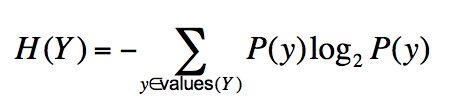
\includegraphics{entropy} \\
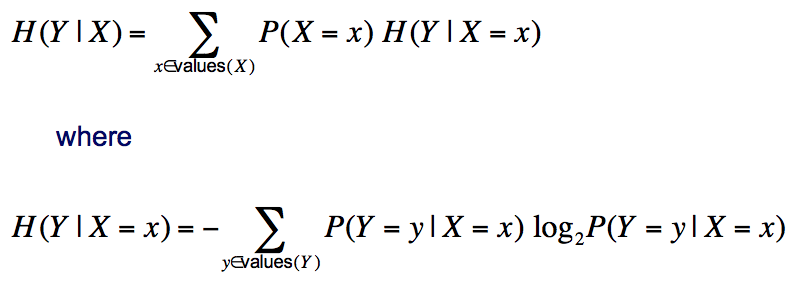
\includegraphics{condentropy}

Information Gain:
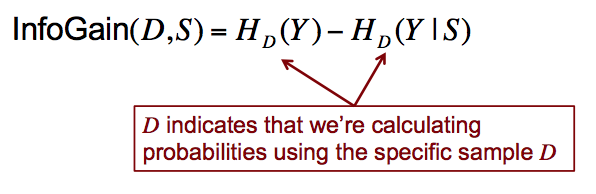
\includegraphics{ig}

Least Squares Regression in CART
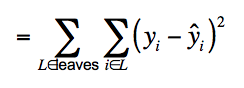
\includegraphics{lsr}

\section{Instance-Based Learning}
\subsection{Goals}
\begin{enumerate}
\item k-NN classification
\item k-NN regression
\item edited nearest neighbor
\item k-d trees for nearest neighbor identification
\item locally weighted regression
\item inductive bias
\end{enumerate}

\subsection{Notes}

\begin{enumerate}
\item Determining similarity/distance
  \begin{enumerate}
    \item Hamming distance: count number of features for which 2
      instances differ (discrete only)
      \item Euclidean distance: $d(x^{(i)},x^{(j)}) =
        \sqrt{\sum_{f}{(x_{f}^{(i)} - x_{f}^{(j)})}^{2}}$
      \item Manhattan distance: $d(x^{(i)},x^{(j)}) =
        \sum_{f}|x_{f}^{(i)} - x_{f}^{(j)}|$
      \item If a mix of continuous/discrete features, refer to equations
      \end{enumerate}
      
\item Normalization
  \begin{itemize}
  \item Determine mean and stddev for feature $x_{i}$ \\
    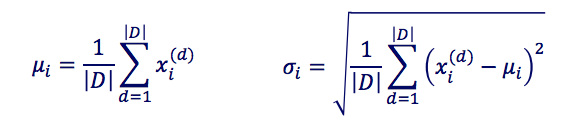
\includegraphics{meanstd}
  \item Standard each feature \\
    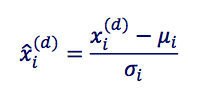
\includegraphics{stand}
  \end{itemize}
  
\item k-NN Regression
  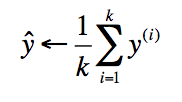
\includegraphics{knnreg}

\item Speeding up k-NN
  \begin{itemize}
  \item Don't retain every training instance
  \item Use smart data structure to look up nearest neighbors (ie k-d
    tree)
  \end{itemize}

\item Edited instance-based learning \\
  \textbf{Incremental deletion}, start will all train inst in memory. If other
  instances provide correct classification for $(x^{(i)},y^{(i)})$,
  delete it \\
  \textbf{Incremental growth}, start with empty memory. If other instances
  don't correctly classify $(x^{(i)},y^{(i)})$, add it to memory

\item k-d trees
  \begin{enumerate}
  \item Similar to DT
  \item Each node stores one instance
  \item Each node splits on median value of feature with highest
    variance
  \item Implemented using priority queue storing nodes considered and
    their lower bound on distance to query instance
  \item k-d trees are sensitive to irrelevant features, \textbf{locally
    weighted regression}
  \end{enumerate}
  Example: \\
  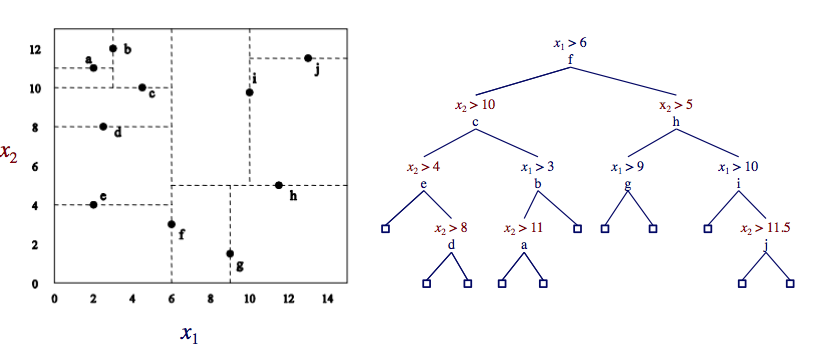
\includegraphics{kd}
  
\item Locally weighted regression \\
  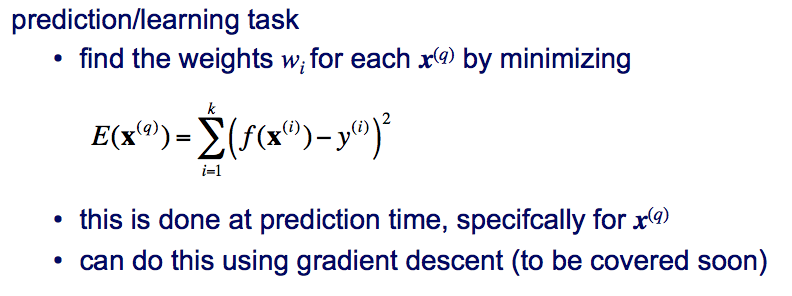
\includegraphics[scale=0.5]{lwr}

\item Stengths of instance-based learning
  \begin{enumerate}
  \item simple to implement
  \item adapts well to online training
  \item robust to noisy training data with k > 1
  \item good in practice
  \end{enumerate}
\item Limits of instance-based learning
  \begin{enumerate}
  \item sensitive to range of feature values
  \item potentially sensitive to irrelevant and correlated features
  \item can be inefficient
  \item no explicit model
  \end{enumerate}
  
\end{enumerate}

\subsection{Equations}

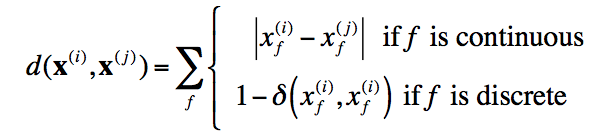
\includegraphics{dist}

\section{ML Methodology}
\subsection{Topics}
\begin{enumerate}
\item bias of an estimator
\item test sets
\item learning curves
\item stratified sampling
\item cross validation
\item confustion matrices
\item TP, FP, TN, FN
\item ROC curves
\item precision-recall curves
\item true positive rate (TPR)
\item positive predictive value (PPV)
\item false positive rate (FPR)
\end{enumerate}

\subsection{Notes}
\begin{enumerate}
\item Bias of an estimator \\
  includegraphics{bias}
\end{enumerate}

\subsection{Equations}
    

\end{document}

